\section{Water Thermal Tanks (includes Water Heaters) }\label{water-thermal-tanks-includes-water-heaters}

Water thermal tanks are devices for storing thermal energy in water.~ The most common types are water heaters. devices for storing and heating water.~ Typical water heater applications are for domestic hot water heating, low-temperature radiant space heating, and energy storage for solar hot water systems or waste heat recovery.~ In EnergyPlus, water heater objects can be coupled to a plant loop simulation or used stand-alone.~ There are also chilled water storage tanks that can be used to hold cold water

\subsection{Mixed Water Thermal Tank}\label{mixed-water-thermal-tank}

The input object WaterHeater:Mixed provides a model that simulates a well-mixed water tank, i.e.~non-stratified, and is appropriate for simulating many types of water heaters and storage tanks, including gas and electric residential water heaters, a variety of large commercial water heaters, and also instantaneous, tankless water heaters.~ This model is used for both the mixed water heater and the mixed chilled water storage tanks.

\subsubsection{Energy Balance}\label{energy-balance}

The well-mixed assumption implies that all water in the tank is at the same temperature.~ To calculate the water temperature, the model analytically solves the differential equation governing the energy balance of the water tank:

\begin{equation}
\rho V{c_p}\frac{{dT}}{{dt}} = {q_{net}}
\end{equation}

where

\emph{r} = density of water

\emph{V} = volume of the tank

\emph{c\(_{p}\)} = specific heat of water

\emph{T} = temperature of the tank water

\emph{t} = time

\emph{q\(_{net}\)} = net heat transfer rate to the tank water

The density and volume can be replaced with the total mass \emph{m} of water in the tank to get:

\begin{equation}
m{c_p}\frac{{dT}}{{dt}} = {q_{net}}
\end{equation}

The net heat transfer rate \emph{q\(_{net}\)} is the sum of gains and losses due to multiple heat transfer pathways.

\begin{equation}
{q_{net}} = {q_{heater}} + {q_{oncycpara}} + {q_{offcycpara}} + {q_{oncycloss}} + {q_{offcycloss}} + {q_{use}} + {q_{source}}
\end{equation}

where

\emph{q\(_{heater}\)} = heat added by the heating element or burner

\emph{q\(_{oncycpara}\)} = heat added due to on-cycle parasitic loads (zero when off)

\emph{q\(_{offcycpara}\)} = heat added due to off-cycle parasitic loads (zero when on)

\emph{q\(_{oncycloss}\)} = heat transfer to/from the ambient environment (zero when off)

\emph{q\(_{offcycloss}\)} = heat transfer to/from the ambient environment (zero when on)

\emph{q\(_{use}\)} = heat transfer to/from the use side plant connections

\emph{q\(_{source}\)} = heat transfer to/from the source side plant connections

\emph{q\(_{oncycloss}\)} and \emph{q\(_{offcycloss}\)} are defined as:

\begin{equation}
{q_{oncycloss}} = U{A_{oncyc}}\left( {{T_{amb}} - T} \right)
\end{equation}

\begin{equation}
{q_{offcycloss}} = U{A_{offcyc}}\left( {{T_{amb}} - T} \right)
\end{equation}

where

\emph{UA\(_{oncyc}\)} = on-cycle loss coefficient to ambient environment (zero when off)

\emph{UA\(_{offcyc}\)} = off-cycle loss coefficient to ambient environment (zero when on)

\emph{T\(_{amb}\)} = temperature of ambient environment

\emph{q\(_{use}\)}, and \emph{q\(_{source}\)} are defined as:

\begin{equation}
{q_{use}} = {\varepsilon_{use}}{\dot m_{use}}{c_p}\left( {{T_{use}} - T} \right)
\end{equation}

\begin{equation}
{q_{source}} = {\varepsilon_{source}}{\dot m_{source}}{c_p}\left( {{T_{source}} - T} \right)
\end{equation}

where

\emph{e\(_{use}\)} = heat exchanger effectiveness for the use side plant connections

\({\dot m_{use}}\) = mass flow rate for the use side plant connections

\emph{T\(_{use}\)} = inlet fluid temperature of the use side plant connections

\emph{e\(_{source}\)} = heat exchanger effectiveness for the source side plant connections

\({\dot m_{source}}\) = mass flow rate for the source side plant connections

\emph{T\(_{source}\)} = inlet fluid temperature of the use side plant connections

Incorporating all of these equations into the original differential equation,

\begin{equation}
  \begin{array}{ll}
    mC_p\frac{dT}{dt} &= q_{heater} + q_{oncyc} + q_{offcyc} + UA_{oncyc} \PB{T_{amb} - T} + UA_{offcyc} \PB{T_{amb} - T} \\ 
                      &+ \varepsilon_{use}\dot{m}_{use}C_p \PB{T_{use} - T} + \varepsilon_{source}\dot{m}_{source}C_p \PB{T_{source} - T}
  \end{array}
\end{equation}

Associating terms not dependent on temperature \emph{T} and terms dependent on temperature \emph{T} yields:

\begin{equation}
  \begin{array}{ll}
    \frac{dT}{dt} &= \RB{\frac{1}{mC_p}\PB{\begin{array}{c}
                                             q_{heater}+q_{oncyc}+q_{offcyc}+UA_{oncyc}T_{amb}+UA_{offcyc}T_{amb} \\
                                             + \varepsilon_{use}\dot{m}_{use}C_pT_{use} + \varepsilon_{source}\dot{m}_{source}C_pT_{source}
                                           \end{array}}} \\
                  &+ \RB{\frac{-1}{mC_p}\PB{UA_{oncyc} + UA_{offcyc}+\varepsilon_{use}\dot{m}_{use}C_p+\varepsilon_{source}\dot{m}_{source}C_p}}T
  \end{array}
\end{equation}

The differential equation now has the form

\begin{equation}
\frac{{dT}}{{dt}} = a + bT
\end{equation}

where

\begin{equation}
a = \frac{1}{{m{c_p}}}\left( \begin{array}{l}{q_{heater}} + {q_{oncyc}} + {q_{offcyc}} + U{A_{oncyc}}{T_{amb}} + U{A_{offcyc}}{T_{amb}}\\ + {\varepsilon_{use}}{{\dot m}_{use}}{c_p}{T_{use}} + {\varepsilon_{source}}{{\dot m}_{source}}{c_p}{T_{source}}\end{array} \right)
\end{equation}

\begin{equation}
b = \frac{{ - 1}}{{m{c_p}}}\left( {U{A_{oncyc}} + U{A_{offcyc}} + {\varepsilon_{use}}{{\dot m}_{use}}{c_p} + {\varepsilon_{source}}{{\dot m}_{source}}{c_p}} \right)
\end{equation}

The solution to the differential equation can be written in terms of \emph{a} and \emph{b} as:

\begin{equation}
T\left( t \right) = \left( {\frac{a}{b} + {T_i}} \right){e^{bt}} - \frac{a}{b}
\end{equation}

where

\emph{T(t)} = temperature of the tank water at time \emph{t}

\emph{T\(_{i}\)} = initial temperature of the tank water at time \emph{t} = 0

However, if \emph{b} = 0, the solution instead is:

\begin{equation}
T\left( t \right) = at + {T_i}
\end{equation}

Since the control algorithm must sometimes calculate the time needed to reach a specified temperature, the equations above can also be rearranged to solve for \emph{t}.

\begin{equation}
t = \frac{1}{b}\ln \left( {\frac{{{\raise0.7ex\hbox{a} \!\mathord{\left/ {\vphantom {a b}}\right.}\!\lower0.7ex\hbox{b}} + {T_f}}}{{{\raise0.7ex\hbox{a} \!\mathord{\left/ {\vphantom {a b}}\right.}\!\lower0.7ex\hbox{b}} + {T_i}}}} \right)
\end{equation}

or, if \emph{b} = 0,

\begin{equation}
t = \frac{{{T_f} - {T_i}}}{a}
\end{equation}

where

\emph{T\(_{f}\)} = final temperature of the tank water at time t.

In the special case where \emph{b} = 0 and \emph{a} = 0, and \emph{T\(_{f}\)} \textless{}\textgreater{} \emph{T\(_{i}\)}, the time \emph{t} is infinity.

\subsubsection{Water Heater Control Algorithm}\label{water-heater-control-algorithm}

For water heaters, control options allow the heater to cycle or modulate to meet the load.~ When cycling, the heater element or burner is either on or off.~ The heater remains fully on while heating the tank up to the setpoint temperature.~ When the setpoint is reached, the heater turns off.~ The heater remains off until the tank temperature falls below the ``cut-in'' temperature, i.e., the setpoint temperature minus the deadband temperature difference.~ The heater continuously cycles on and off to maintain the tank temperature within the deadband.~ Most storage-tank water heaters cycle.

When modulating, the heater power varies between the maximum and minimum heater capacities.~ The heater stays on as long as the required total demand is above the minimum capacity.~ Below the minimum capacity, the heater will begin to cycle on and off based on the deadband temperature difference.~ Most tankless/instantaneous water heaters modulate.

Within a time step, the differential equation is solved separately for when the heater element or burner is ``on'' (on-cycle) and when it is ``off'' (off-cycle).~ This approach allows ambient losses and parasitic loads to be divided into on-cycle and off-cycle effects and accounted for in detail.

An illustration of how the control algorithm cycles on and off is shown below.~ Ambient losses cool the tank temperature until the bottom of the deadband is reached (50 C) at which point the heater cycles on and reheats the tank back to the setpoint (60 C).~ A water draw causes hot water to be replaced with cold water from the water mains.~ The incoming cold water rapidly cools the tank.~ In this example the heater cannot keep up with the water draw and the tank temperature continues to drop until the water draw ends.

Although the instantaneous tank water temperature may vary considerably within a timestep (due to cycling, etc.), only the average temperature over the timestep is reported.~ The model calculates the average by piece-wise integration of the area under the instantaneous temperature curve for each unique set of conditions.~ The instantaneous temperature is preserved internally by the program and is propogated from the end of one timestep to the beginning of the next.

\begin{figure}[hbtp] % fig 311
\centering
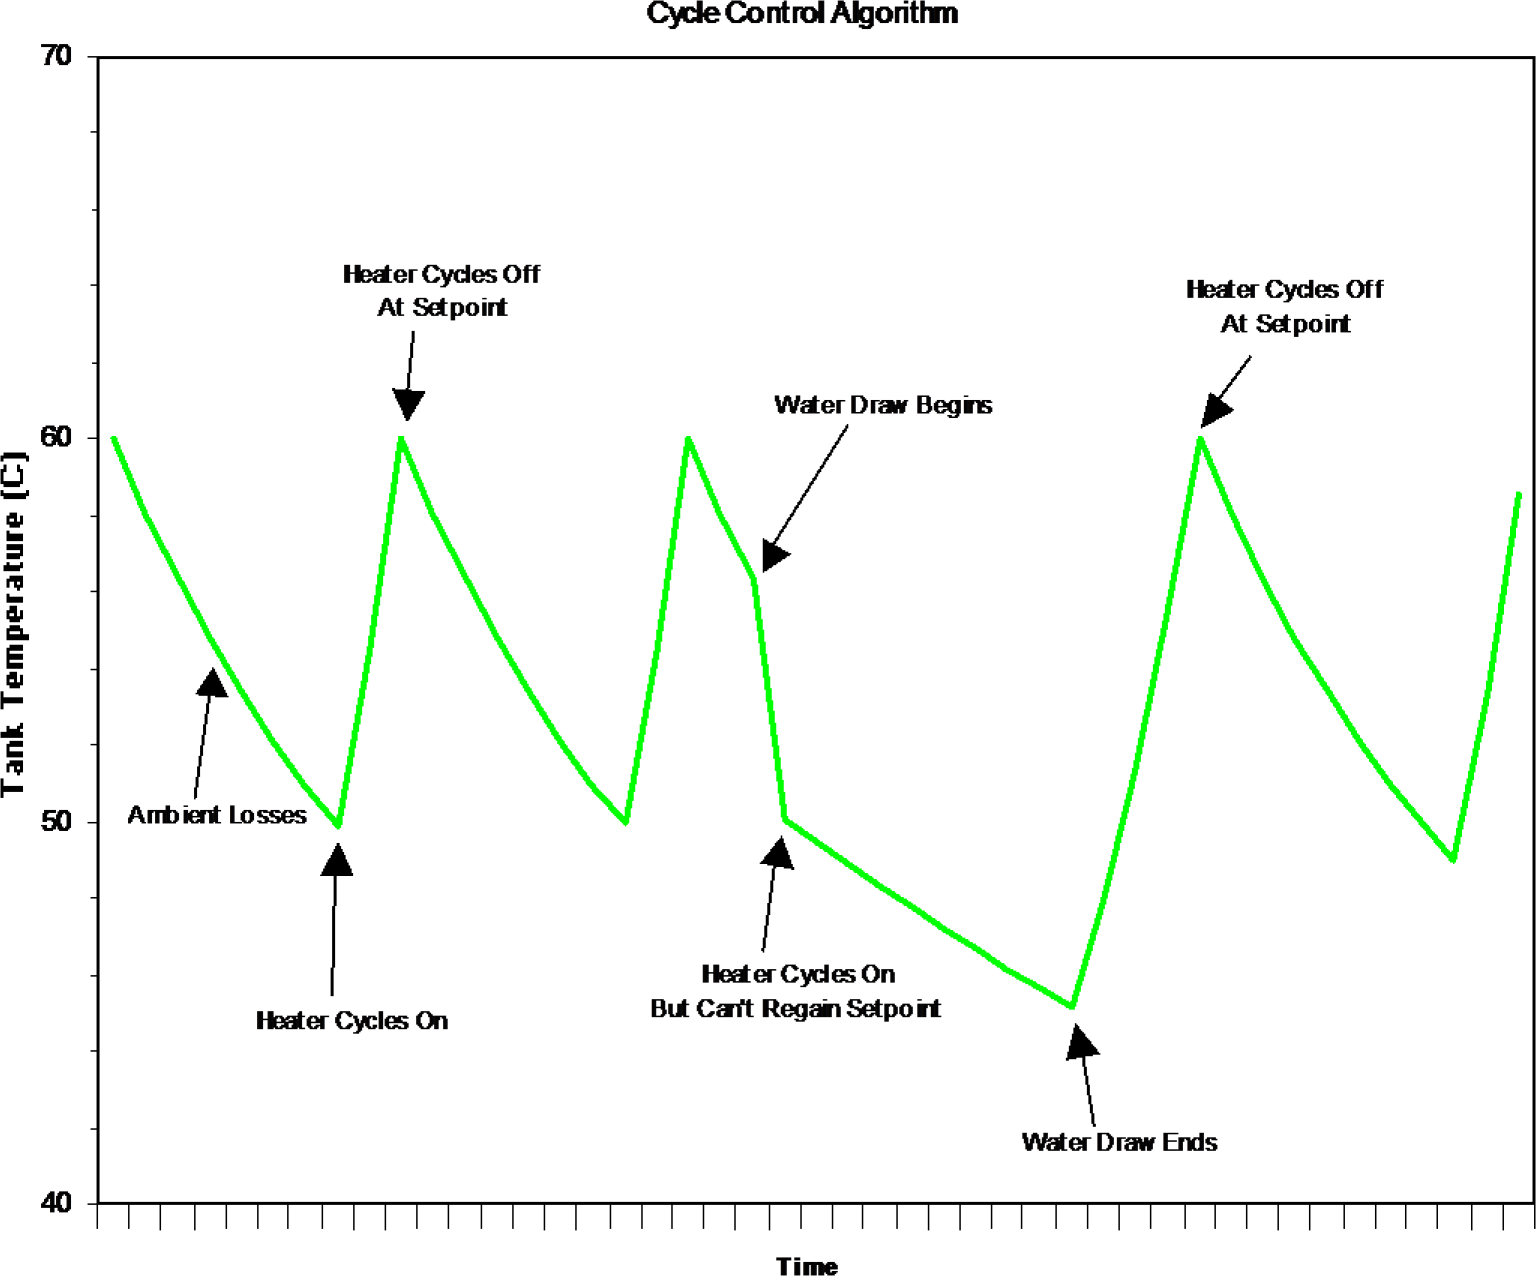
\includegraphics[width=0.9\textwidth, height=0.9\textheight, keepaspectratio=true]{media/image6852.png}
\caption{Water Heater Cycle Control Algorithm \protect \label{fig:water-heater-cycle-control-algorithm}}
\end{figure}

\subsubsection{Chilled Water Tank Control Algorithm}\label{chilled-water-tank-control-algorithm}

The input objects ThermalStorage:ChilledWater:Mixed and ThermalStorage:ChilledWater:Stratified provide chilled water tank models that do not include active cooling elements, there is only indirect cooling by remote devices such as a chiller.~ The tank's setpoint controls are used to determine if flow is to be requested through the source side of the tank.~ The setpont and deadband control scheme is similar to the water heater but the logic is flipped around for cooling instead of heating.~ The setpoint temperatue is the ``cut-out'' temperature and the setpoint plus deadband is the ``cut-in'' temperature.~ If the tank temperature ( or tank sensing node for stratified tanks) is above the ``cut-in'' temperature, then flow is requested.~ If temperatures are below the ``cut-out'' temperature, then flow is not requested.~ The chilled water tanks also have separate availability schedules for the use side and source side for additional control options.

\subsubsection{Standard Ratings}\label{standard-ratings-000}

For water heaters, the industry standard ratings of Recovery Efficiency and Energy Factor are calculated according to the 10CFR430 test procedure.~ To emulate the test procedure, a 24-hour simulation of the water heater is performed internally using the specified test conditions:

n~Setpoint Temperature = 57.2 C (135 F)

n~Ambient Temperature = 19.7 C (67.5 F)

n~Ambient Relative Humidity = 50\% (used for heat pump water heaters)

n~Inlet Temperature (Water Mains) = 14.4 C (58 F)

For heat pump water heaters, the water heater tank's heating element and water heater tank parasitic loads are disabled and the user-defined water heating capacity, energy use, and parasitic loads for the heat pump are used to calculate Recovery Efficiency and Energy Factor.

The simulated test procedure performs six equal draws of approximately 0.041 m\(^{3}\) (10.7 gal) in each of the first six hours of the simulation.~ Each draw occurs over the first timestep of the hour.

The Recovery Efficiency is calculated when the water heater recovers to the setpoint after the first draw.

\begin{equation}
RE = \frac{{{m_1}{c_p}\left( {57.2 - 14.4} \right)}}{{{E_1}}}
\end{equation}

where

\emph{m\(_{1}\)} = water mass of the first draw

\emph{c\(_{p}\)} = specific heat of water

\emph{E\(_{1}\)} = fuel energy consumed until the setpoint is recovered (including parasitics)

Note: When the standards rating for a heat pump water heater is calculated, the fuel energy consumed refers to the total energy consumed by the heat pump compressor, evaporator fan, condenser pump, and parasitic loads. It is assumed that the parasitic loads for a heat pump water heater do not contribute to heating the water (ref. Heat Pump Water Heater).

The Energy Factor is calculated at the end of the 24-hour simulation period.

\begin{equation}
EF = \frac{{{m_{total}}{c_p}\left( {57.2 - 14.4} \right)}}{{{E_{total}}}}
\end{equation}

where

\emph{m\(_{total}\)} = total water mass of all six draws

\emph{c\(_{p}\)} = specific heat of water

\emph{E\(_{total}\)} = total fuel energy consumed over 24 hours (including parasitics)

Under certain input parameters, the rating method will not succeed and a warning message will be generated.~ Problems occur when inputs do not allow the tank to recover to the setpoint temperature within the test period.~ This can occur if the maximum heater capacity is undersized, or if the deadband temperature difference is large enough that the first draw of the test does not trigger the heater to come on.~ In either case, the Recovery Efficiency test will not compute properly because recovery to the setpoint was not achieved.

\subsubsection{References}\label{references-053}

10CFR430.~ \emph{Title 10, Code of Federal Regulations, Part 430 - Energy Conservation Program for Consumer Products, Appendix E to Subpart B - Uniform Test Procedure for Measuring the Energy Consumption of Water Heaters}.

\subsection{Heat Pump Water Heater}\label{heat-pump-water-heater}

\subsubsection{Overview}\label{overview-029}

The input objects \lstinline!WaterHeater:HeatPump:*! provide models for a heat pump water heater (HPWH) that is a compound object consisting of a water heater tank (e.g., \lstinline!WaterHeater:Mixed! or \lstinline!WaterHeater:Stratified!), a direct expansion (DX) ``coil'' (i.e., an air-to-water DX compression system which includes a water heating coil, air coil, compressor, and water pump), and a fan to provide air flow across the air coil associated with the DX compression system. These objects work together to model a system which heats water using zone air, outdoor air, or a combination of zone and outdoor air as the primary heat source.

There are two types of heat pump water heater models available:

\begin{enumerate}
\def\labelenumi{\arabic{enumi}.}
\tightlist
\item
  \lstinline!WaterHeater:HeatPump:PumpedCondenser!: This model is used to represent a heat pump water heater where water is removed from the tank, pumped through a condenser, and returned to the tank at a higher temperature.
\item
  \lstinline!WaterHeater:HeatPump:WrappedCondenser!: This model is used for heat pump water heaters that are more typical in the residential building context where the heating coil is wrapped around or submerged in the tank.
\end{enumerate}

Each type of \lstinline!WaterHeater:HeatPump:*! object is compatible with certain \lstinline!Coil:WaterHeating:AirToWaterHeatPump:*! objects as shown in the following table:

\begin{longtable}[c]{@{}ll@{}}
\toprule 
WaterHeater:HeatPump:* & WaterHeater:* \tabularnewline
\midrule
\endfirsthead

\toprule 
WaterHeater:HeatPump:* & WaterHeater:* \tabularnewline
\midrule
\endhead

PumpedCondenser & Pumped \tabularnewline
PumpedCondenser & VariableSpeed \tabularnewline
WrappedCondenser & Wrapped \tabularnewline
\bottomrule
\end{longtable}

Additionally the \lstinline!WaterHeater:HeatPump:WrappedCondenser! object is only compatible with stratified tanks. Therefore \lstinline!WaterHeater:HeatPump:*! has the following tank compatibility matrix:

\begin{longtable}[c]{@{}lll@{}}
\toprule
WaterHeater:HeatPump:* & \multicolumn{2}{c}{WaterHeater:*} \tabularnewline
\cmidrule{2-3}
& Mixed & Stratified \tabularnewline
\midrule
\endhead

Pumped & X & X \tabularnewline
Wrapped &  & X \tabularnewline
\bottomrule
\end{longtable}

Numerous configurations of tank location, inlet air source, and DX coil compressor location can be modeled. The DX coil compressor may be located in a zone, outdoors, or the ambient temperature surrounding the compressor may be scheduled. The location of the compressor controls the operation of its crankcase heater. The water heater tank location is specified in the water heater tank object and is independent of the compressor location. In addition, the inlet air configuration may be specified in one of several ways. The heat pump water heater air coil and fan assembly may draw its inlet air from the zone and outdoor air using an optional mixer and splitter assembly as shown in the first figure below. When used, the mixer and splitter air streams are controlled by a single inlet air mixer schedule. When the HPWH draws its inlet air solely from a zone, the mixer/splitter assembly is not required as shown in the second figure below. In this case, the inlet air to the evaporator and fan assembly is made up entirely of zone air and the heat pump outlet air is directed back to the zone. The final figure illustrates a HPWH that draws its inlet air solely from outdoors and exhausts its outlet air outdoors as well. Each of these configurations may also be connected to a plant hot water loop (via the water heater tank use nodes).

\begin{figure}[hbtp] % fig 312
\centering
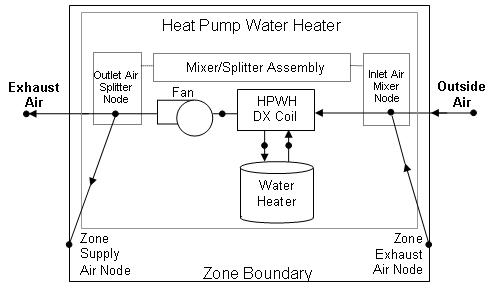
\includegraphics[width=0.9\textwidth, height=0.9\textheight, keepaspectratio=true]{media/image6855.png}
\caption{Schematic of a heat pump water heater using optional mixer/splitter nodes \protect \label{fig:schematic-of-a-heat-pump-water-heater-using-001}}
\end{figure}

\begin{figure}[hbtp] % fig 313
\centering
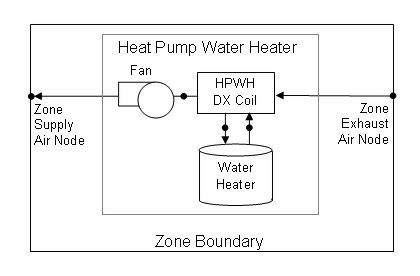
\includegraphics[width=0.9\textwidth, height=0.9\textheight, keepaspectratio=true]{media/image6856.png}
\caption{Schematic of a Heat Pump Water Heater with Inlet Air from a Zone \protect \label{fig:schematic-of-a-heat-pump-water-heater-with}}
\end{figure}

\begin{figure}[hbtp] % fig 314
\centering
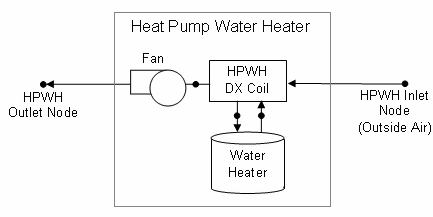
\includegraphics[width=0.9\textwidth, height=0.9\textheight, keepaspectratio=true]{media/image6857.png}
\caption{Schematic of a Heat Pump Water Heater with Inlet Air from Outdoors \protect \label{fig:schematic-of-a-heat-pump-water-heater-with-001}}
\end{figure}

Note: The water heater tank location shown in the figures above is completely independent of the heat pump water heater's inlet air configuration and its compressor location. The water heater tank may be located outdoors, in a zone, or the ambient temperature surrounding the tank can be scheduled as described in the mixed water heater section below.

\subsubsection{Model Description}\label{model-description-016}

The heat pump water heater input requires a compressor setpoint temperature schedule and dead band temperature difference, which are independent from the setpoint temperature schedule and dead band temperature difference for the heater (element or burner) associated with the water heater tank. The cut-in temperature for the heat pump compressor is defined as the heat pump compressor's setpoint temperature minus its dead band temperature difference.

\begin{equation}
{T_{HP,\,cut - in}}\,\, = \,\,{T_{HP,set\,point}}\,\, - \,\,{T_{HP,dead\,band}}
\end{equation}

where:

\({T_{HP,\,cut - in}}\) ~~~~ = Cut-in temperature for the heat pump compressor (°C)

\({T_{HP,set\,point}}\) ~~ = Heat pump compressor setpoint temperature (°C)

\({T_{HP,dead\,band}}\) = Heat pump compressor dead band temperature difference (°C)

In this model, the heat pump water heater's DX compression system is considered the primary heat source and the water tank's heater (element or burner) provides supplemental heat as necessary. Therefore, the cut-in temperature for the heat pump compressor (setpoint minus dead band temperature difference) is usually higher than the setpoint temperature for the heater (element or burner) in the associated water heater tank object. At times when the water heater tank setpoint temperature is greater than the cut-in temperature of the heat pump compressor, the heat pump compressor is disabled and the tank's heater is used to heat the water.

The simulation starts by first calculating the air conditions entering the air coil (evaporator)/fan assembly based on the inlet air configuration of the heat pump water heater and the presence of the optional mixer/splitter nodes. When the HPWH draws its inlet air from the zone and outdoors using the optional mixer/splitter nodes (i.e., Inlet Air Configuration = Zone and Outdoor Air), the inlet air conditions are calculated as follows:

\begin{equation}
Frac = GetScheduleValue(MixerInletAirSchedule)
\end{equation}

\begin{equation}
{T_{inlet}} = {T_{outdoor}}\left( {Frac} \right) + {T_{zone}}\left( {1 - Frac} \right)
\end{equation}

\begin{equation}
{\omega_{inlet}} = {\omega_{outdoor}}\left( {Frac} \right) + {\omega_{zone}}\left( {1 - Frac} \right)
\end{equation}

where:

\(Frac\) ~ = current value of the inlet air mixer schedule (fraction of outdoor air, 0-1)

\({T_{inlet}}\) ~ = inlet air dry-bulb temperature to the HPWH evaporator/fan assembly (°C)

\({T_{outdoor}}\) ~ = outdoor air dry-bulb temperature (°C)

\({T_{zone}}\) ~ = zone (exhaust) air dry-bulb temperature (°C)

\({\omega_{inlet}}\) ~ = inlet air humidity ratio to the HPWH evaporator/fan assembly (kg/kg)

\({\omega_{outdoor}}\) = outdoor air humidity ratio (kg/kg)

\({\omega_{zone}}\) ~ = zone (exhaust) air humidity ratio (kg/kg)

When the heat pump water heater draws its inlet air solely from the zone (i.e., Inlet Air Configuration = Zone Air Only), the inlet air conditions to the evaporator/fan assembly are simply set equal to the zone (exhaust) air conditions. If the heat pump water heater draws its inlet air solely from outdoors (i.e., Inlet Air Configuration = Outdoor Air Only), the inlet air conditions to the evaporator/fan assembly are simply set equal to the outdoor air conditions. When the inlet air to the heat pump water heater evaporator and fan assembly is scheduled (i.e., Inlet Air Configuration = Schedule), the inlet air conditions are determined directly from the user-supplied schedules as follows.

\begin{equation}
{T_{inlet}} = GetScheduleValue(InletAirTemperatureSchedule)
\end{equation}

\begin{equation}
RHinlet = GetScheduleValue(InletAirHumiditySchedule)
\end{equation}

\begin{equation}
{\omega_{inlet}} = PsyWFnTdbRhPb({T_{inlet}},R{H_{inlet}},OutBaroPress)
\end{equation}

where:

\(R{H_{inlet}}\) = inlet air relative humidity to heat pump water heater evaporator/fan assembly (0-1)

\(PsyWFnTdbRhPb\) = psychrometric function returning air humidity ratio given dry-bulb temperature, relative humidity, and barometric pressure

\(OutBaroPress\) = outdoor barometric pressure (Pa)

For each simulation time step, the heat pump water heating capacity, energy use, and air-side/water-side mass flow rates are set to zero and the water heater tank is simulated with the heat pump compressor disabled when any of the following conditions apply:

·~~~~~~~~the HPWH is scheduled off by its availability schedule,

·~~~~~~~~the water heater tank setpoint temperature is greater than or equal to the heat pump compressor cut-in temperature,

·~~~~~~~~the inlet air dry-bulb temperature to the evaporator/fan assembly is less than the Minimum Inlet Air Temperature for Heat Pump Compressor Operation (as specified by the user in the HPWH input object), or

·~~~~~~~~the HPWH setpoint temperature is greater than or equal to the Maximum Temperature Limit (specified in the Water Heater:Mixed object).

Otherwise, simulation of the heat pump water heater is based on its current mode of operation. This mode of operation is either floating (heat pump compressor is off and tank water temperature has not fallen below the heat pump compressor cut-in temperature) or heating (tank water temperature dropped below the compressor cut-in temperature on a previous time step but was unable to reach the compressor setpoint temperature). Each mode is handled differently and they will be discussed separately.

If the heat pump water heater is using the stratified tank model, then there is more than one value for the tank temperature.~ The model includes input for where the heat pump controls detect the temperature. The input data in the associated WaterHeater:Stratified includes up to two heights in the tank where the temperature is measured and a weight associated with each. The associated stratified tank nodes are selected based on these heights. When the heat pump model needs to evaluate the tank temperature of a stratified tank, it evaluates the temperature at the tank nodes associated with these locations.

\subsubsection{Float Mode}\label{float-mode-000}

When the heat pump water heater tank temperature is floating between the heat pump compressor's cut-in and cut-out temperatures at the end of the previous simulation time step, both the heat pump compressor and the water heater tank's heating element are disabled and a resulting tank temperature is calculated. If the resulting tank temperature is below the heat pump compressor's cut-in temperature, the heat pump compressor part-load ratio is estimated using the ratio of the temperature differences shown below. The part-load ratio can not be less than zero or greater than one.

\begin{equation}
PLR = MIN\left( {1.0,\,\,MAX\left( {0.0,\,\,\left( {\frac{{{T_{HP,\,cut - in}} - {T_{tank,float}}}}{{{T_{tank,initial}} - {T_{tank,float}}}}} \right)} \right)} \right)
\end{equation}

where:

\(PLR\) ~~~~~~~~ = part-load ratio of the heat pump water heater compressor

\(Ttank,float\) ~~~ = tank temperature in float mode when heating capacity is set to zero(°C)

\({T_{tank,initial}}\) ~~~ = tank temperature at the beginning of the simulation time step (°C)

Since the pump and fan are assumed to cycle on and off with the heat pump compressor, the average condenser water (for pumped condensers only) and evaporator air mass flow rates for the simulation time step are calculated based on the PLR calculated above:

\begin{equation}
{\dot m_{water,avg}} = \dot Vwater\left( {{\rho_{water}}} \right)\left( {PLR} \right)
\end{equation}

\begin{equation}
\dot mair,avg = \dot Vair\left( {{\rho_{air}}} \right)\left( {PLR} \right)
\end{equation}

where:

\(\dot mwater,avg\) ~~~~~~ = average condenser water mass flow rate for the time step (kg/s)

\(\dot Vwater\) ~~~~~~~~~~~ = condenser water volumetric flow rate, user input (m\(^{3}\)/s)

\({\rho_{water}}\) ~~~~~~~~~~~ = density of condenser inlet water (kg/m\(^{3}\))

\(\dot mair,avg\) ~~~~~~~~ = average evaporator/fan air mass flow rate for the time step (kg/s)

\(\dot Vair\) ~~~~~~~~~~~~~~ = evaporator/fan air volumetric flow rate, user input (m\(^{3}\)/s)

\({\rho_{air}}\) ~~~~~~~~~~~~~ = density of evaporator/fan inlet air (kg/m\(^{3}\))

The water tank temperature is then calculated based on heat pump operation at the part-load ratio estimated above and with the water tank's heating element enabled. If the resulting water tank temperature is above the heat pump compressor's setpoint (cut-out) temperature, then the part-load ratio is reduced and the water heater tank is simulated again. The process is performed iteratively until the part-load ratio of the heat pump compressor achieves the desired setpoint temperature (to the extent possible).

\subsubsection{Heating Mode}\label{heating-mode-000}

When the HPWH is in heating mode at the end of the previous simulation time step (i.e., the heat pump compressor operated during the previous simulation time step but was unable to achieve the setpoint temperature), both the heat pump compressor and the water heater tank's heating element are enabled. The part-load ratio of the heat pump compressor is set to 1, and the condenser water (for pumped condensers) and evaporator air mass flow rates are set to their maximum flow rates.

\begin{equation}
{\dot m_{water,avg}} = {\dot V_{water}}\left( {{\rho_{water}}} \right)
\end{equation}

\begin{equation}
\dot mair,avg = \dot Vair\left( {\rho air} \right)
\end{equation}

If the resulting tank temperature is above the heat pump compressor's setpoint (cut-out) temperature, the part-load ratio of the heat pump compressor is reduced and the water heater tank is simulated again. The process is performed iteratively until the part-load ratio of the heat pump compressor achieves the desired setpoint temperature (to the extent possible).

The air-side outlet conditions of the HPWH are calculated through simulation of the fan and DX coil with either a blow through or draw through fan placement (user selectable). If mixer/splitter nodes are used, the HPWH model splits the heat pump outlet air mass flow rate with exhaust air flow equaling the outdoor air flow, and the balance of the outlet air being sent to the zone supply air node (i.e., ensures that the heat pump water heater does not contribute to zone pressurization or depressurization). Calculations of heat pump water heating capacity, energy use, air-side performance, and water-side temperature difference are performed in the associated DX Coil object. See the engineering reference section for the Coil:WaterHeating:AirToWaterHeatPump object for details.

\subsubsection{Model Outputs}\label{model-outputs-000}

After completing the float mode or heating mode calculations and the final part-load ratio has been determined, the output (report) variables are calculated as follows:

\begin{equation}
Heat\,Pump\,Water\,Heater\,Compressor\,Part{\rm{ - }}Load\,Ratio = PLR\,\,
\end{equation}

\begin{equation}
Heat\,Pump\,Water\,Heater\,\,On{\rm{ - }}Cycle\,Parasitic\,Electric\,Power\,(W)\,\, = \,\,{P_{parasitic,on}}\left( {PLR} \right)
\end{equation}

\begin{equation}
\begin{split}
Heat\,Pump\,Water\,Heater\,\,On{\rm{ - }}Cycle\,Parasitic\,Electric\,Consumption\,(J)\,\, = \\{P_{parasitic,on}}\left( {PLR} \right)\left( {3600} \right){t_{sys}}
\end{split}
\end{equation}

\begin{equation}
\begin{split}
Heat\,Pump\,Water\,Heater\,\,Off{\rm{ - }}Cycle\,Parasitic\,Electric\,Power\,(W)\,\, = \\{P_{parasitic,off}}\left( {1 - PLR} \right)
\end{split}
\end{equation}

\begin{equation}
\begin{split}
Heat\,Pump\,Water\,Heater\,\,Off{\rm{ - }}Cycle\,Parasitic\,Electric\,Consumption\,(J)\,\, = \\{P_{parasitic,off}}\left( {1 - PLR} \right)\left( {3600} \right)\left( {{t_{sys}}} \right)
\end{split}
\end{equation}

where:

\({P_{parasitic,on}}\) ~~ = on-cycle parasitic electric load, user input (W)

\({P_{parasitic,off}}\) ~ = off-cycle parasitic electric load, user input (W)

\({t_{sys}}\) ~~~~~~~~~~~~ = HVAC system simulation time step (hours)

Note: All heat pump water heater output variables, including off-cycle ancillary electric power and consumption, equal 0 when the heat pump water heater availability schedule equals 0 (i.e., the heat pump water heater is scheduled OFF).

\subsection{Stratified Water Thermal Tank}\label{stratified-water-thermal-tank}

The input objects WaterHeater:Stratified and ThermalStorage:ChilledWater:Stratified provide models for a stratified water thermal tank that divides the water tank into multiple nodes of equal volume.~ This model is used for both the stratified water heater and the stratified chilled water storage tank. The nodes are coupled by vertical conduction effects, internode fluid flow, and temperature inversion mixing.~ The object simultaneously solves the differential equations governing the energy balances on the nodes using the Forward-Euler numerical method.~ The system time step is divided into one second substeps that allow the simulation to capture events that occur on a very short time scale.

\subsubsection{Energy Balance}\label{energy-balance-1}

Similar to the well-mixed model, the stratified model solves the same fundamental differential equation governing the energy balance on a mass of water:

\begin{equation}
m{c_p}\frac{{dT}}{{dt}} = {q_{net}}
\end{equation}

where

\emph{m} = mass of water

\emph{c\(_{p}\)} = specific heat of water

\emph{T} = temperature of water

\emph{t} = time

\emph{q\(_{net}\)} = net heat transfer rate

The difference for the stratified model is that it must solve the energy balance on \emph{n} number of nodes simultaneously.~ Node 1 is at the top of the water tank and node \emph{n} is at the bottom of the water tank.

\begin{equation}
{m_n}{c_p}\frac{{d{T_n}}}{{dt}} = {q_{net,n}}
\end{equation}

where

\emph{m\(_{n}\)} = mass of water for node \emph{n}

\emph{c\(_{p}\)} = specific heat of water

\emph{T\(_{n}\)} = temperature of water for node \emph{n}

\emph{t} = time

\emph{q\(_{net,n}\)} = net heat transfer rate for node \emph{n}

The net heat transfer rate \emph{q\(_{net}\)} is the sum of gains and losses due to multiple heat transfer pathways.

\begin{equation}
  \begin{array}{ll}
    q_{net,n} &= q_{heater,n} + q_{oncycpara,n} + q_{offcycpara,n} + q_{oncycloss,n} + q_{offcycloss,n} \\ 
              &+ q_{cond,n} + q_{use,n} + q_{source,n} + q_{flow,n} + q_{invmix,n}
  \end{array}
\end{equation}

where

\emph{q\(_{heater,n}\)} = heat added by Heater 1 or Heater 2

\emph{q\(_{oncycpara,n}\)} = heat added due to on-cycle parasitic loads (zero when off)

\emph{q\(_{offcycpara,n}\)} = heat added due to off-cycle parasitic loads (zero when on)

\emph{q\(_{oncycloss,n}\)} = heat transfer to/from the ambient environment (zero when off)

\emph{q\(_{offcycloss,n}\)} = heat transfer to/from the ambient environment (zero when on)

\emph{q\(_{cond,n}\)} = heat transfer due to conduction between the node above and below

\emph{q\(_{use,n}\)} = heat transfer to/from the use side plant connections

\emph{q\(_{source,n}\)} = heat transfer to/from the source side plant connections

\emph{q\(_{flow,n}\)} = heat transfer due to fluid flow from the node above and below

\emph{q\(_{invmix,n}\)} = heat transfer due to inversion mixing from the node above and below

\emph{q\(_{oncycloss,n}\)} and \emph{q\(_{offcycloss,n}\)} are defined as:

\begin{equation}
{q_{oncycloss,n}} = ({UA_{tank}} + UA_add,n)({T_{amb}} - {T_n})
\end{equation}

\begin{equation}
{q_{offcycloss,n}} = ({UA_{tank} + UA_{flue}})({T_{amb}} - {T_n})
\end{equation}

where

\emph{UA\(_{tank}\)} = loss coefficient to ambient environment for the tank

\emph{UA\(_{add,n}\)} = additional node loss coefficient

\emph{UA\(_{flue}\)} = additional off-cycle flue loss coefficient to ambient environment (zero when on)

\emph{T\(_{amb}\)} = temperature of ambient environment

\emph{q\(_{cond,n}\)} is defined as:

\begin{equation}
{q_{cond,n}} = \frac{{k{A_{n + 1}}}}{{{L_{n + 1}}}}({T_{n + 1}} - {T_n}) + \frac{{k{A_{n - 1}}}}{{{L_{n - 1}}}}({T_{n - 1}} - {T_n})
\end{equation}

where

\emph{k} = fluid thermal conductivity of water, 0.6 W/m-K

\emph{A\(_{n+1}\)} = shared surface area between node \emph{n} and node \emph{n+1}

\emph{L\(_{n+1}\)} = distance between the center of mass of node \emph{n} and n\emph{+1}

\emph{T\(_{n+1}\)} = temperature of node \emph{n+1}

\emph{A\(_{n-1}\)} = shared surface area between node \emph{n} and node \emph{n-1}

\emph{L\(_{n-1}\)} = distance between the center of mass of node \emph{n} and n\emph{-1}

\emph{T\(_{n-1}\)} = temperature of node \emph{n-1}

\emph{q\(_{use,n}\)}, and \emph{q\(_{source,n}\)} are defined as:

\begin{equation}
{q_{use}} = {\varepsilon_{use}}{\dot m_{use}}{c_p}\left( {{T_{use}} - T} \right)
\end{equation}

\begin{equation}
{q_{source}} = {\varepsilon_{source}}{\dot m_{source}}{c_p}\left( {{T_{source}} - T} \right)
\end{equation}

where

\emph{e\(_{use}\)} = heat exchanger effectiveness for the use side plant connections

\({\dot m_{use}}\) = mass flow rate for the use side plant connections

\emph{T\(_{use}\)} = inlet fluid temperature of the use side plant connections

\emph{e\(_{source}\)} = heat exchanger effectiveness for the source side plant connections

\({\dot m_{source}}\) = mass flow rate for the source side plant connections

\emph{T\(_{source}\)} = inlet fluid temperature of the source side plant connections

\emph{q\(_{flow,n}\)} is defined as:

\begin{equation}
{q_{flow,n}} = {\dot m_{n + 1}}{c_p}({T_{n + 1}} - {T_n}) + {\dot m_{n - 1}}{c_p}({T_{n - 1}} - {T_n})
\end{equation}

where

\({\dot m_{n + 1}}\) = mass flow rate from node \emph{n+1}

\({\dot m_{n - 1}}\) = mass flow rate from node \emph{n-1}

\emph{q\(_{invmix,n}\)} is defined as:

\begin{equation}
{q_{invmix,n}} = {\dot m_{invmix,n + 1}}{c_p}({T_{n + 1}} - {T_n}) + {\dot m_{invmix,n - 1}}{c_p}({T_{n - 1}} - {T_n})
\end{equation}

where

\({\dot m_{invmix,n + 1}}\) = mass flow rate from node \emph{n+1} due to temperature inversion mixing

\({\dot m_{invmix,n - 1}}\) = mass flow rate from node \emph{n-1} due to temperature inversion mixing

Inversion mixing occurs when the node below is warmer than the node above.~ The difference in temperatures drives a difference in density that causes the nodes to mix.~ Usually inversion mixing occurs very rapidly.~ In this algorithm, the inversion mixing rate is selected to be the maximum value that will provide a stable solution given the node mass and the substep interval:

\begin{equation}
{\dot m_{invmix}} = 0.5*{m_n}/\Delta t
\end{equation}

where

\emph{Dt} = the substep time interval.

The use and source fluid steam outlet temperatures calculation procedure depends on the values of the effectiveness.~ If the effectiveness is 1.0, then complete mixing of these fluid steam and the tank water is assumed.~ In this case the outlet temperatures for the use and source streams will be simply the tank water temperatures at point of the outlet nodes. When the effectiveness is less than 1.0, an indirect heat exchange is assumed between the use or source stream and the water in the stratified thermal storage tank.~ When the effectiveness is less than 1.0, the use and source outlet temperatures are calculated using \emph{Q\(_{use}\)} and \emph{Q\(_{source}\)}, and energy balance equations as follows:

\begin{equation}
{T_{use\;out,\,n}} = {T_{use,\,n}} + \frac{{{q_{use,n}}}}{{{{\dot m}_{use}}{c_p}}}
\end{equation}

\begin{equation}
{T_{source\;out,\,n}} = {T_{source,\,n}} - \frac{{{q_{source,n}}}}{{{{\dot m}_{source}}{c_p}}}
\end{equation}

~where,

\emph{T\(_{use\, out}\)} = outlet fluid temperature of the use side plant connections

\emph{T\(_{source\, out}\)} = outlet fluid temperature of the source side plant connections

\subsubsection{Numerical Solution}\label{numerical-solution}

The system of simultaneous differential equations is solved using the Forward-Euler numerical method.~ The system time step is divided into one-second substeps.~ The new temperature for a given node is calculated using the following equation:

\begin{equation}
{T_n} = {T_{n,old}} + \frac{{{q_{net,n}}\Delta t}}{{{m_n}{c_p}}}
\end{equation}

All node temperatures for \emph{q\(_{net,n}\)} are the old temperatures from the previous substep.

Before each system time step is calculated the following evaluations are made:

§~Use and source inlet flow rates are applied to the inlet nodes

§~Internode flow is determined and net flow rates are determined

Before each substep is calculated, the following evaluations are made:

1)~~~Thermostatic controls for heater 1 and heater 2 are evaluated to determine if the heater elements should turn on or off

2)~~~Node 1 temperature is compared against the maximum limit to determine if venting is necessary

3)~~~Adjoining node temperatures are compared to determine if there are any temperature inversions for which the inversion mixing rate should be used.

The solution continues looping through all substeps until the system time step is completed.

\subsubsection{References}\label{references-1-017}

Duffie, J., and W. Beckman. 1980. \emph{Solar Engineering of Thermal Processes}.~ John Wiley \& Sons.

Newton, B. 1995. \emph{Modeling of Solar Storage Tanks}.~ Master's Dissertation, University of Wisconsin-Madison.

\subsection{Water Heating Sizing}\label{water-heating-sizing}

Some inputs for water heaters can be autosized using the input object WaterHeater:Sizing.~ This section describes the sizing calculations for water heaters.~ There are six general methods for sizing tank volume and heating capacity.

\subsubsection{Autosizing Tank Volume}\label{autosizing-tank-volume}

The volume a water heater can be sized in the following ways depending on the design method chosen by the user.

\begin{itemize}
  \item Peak Draw. The volume is determined from the loop design flow rate.~ The water heater is positioned on the supply side of a plant loop.~ After the plant sizing routines have run, the model~ obtains the design flow rate for all components on the demand side.~ The tank volume is then: \(V = {\dot V_{loop.des}}*{t_{draw}}\) ,

  \item Residential HUD-FHA Minimum. The volume is determined from a set of rules defined by the table below.~ This is from Chapter 48 of 1999 ASHRAE Handbook HVAC Applications, Americal Society of Heating Refrigeration and Air-conditioning Engineeers, Atlanta GA.~ (also used in the Building America Benchmark).
\end{itemize}

% table 85
{\scriptsize
\begin{longtable}[c]{>{\raggedright}p{0.8in}p{0.35in}p{0.35in}p{0.35in}p{0.35in}p{0.35in}p{0.35in}p{0.35in}p{0.35in}p{0.35in}p{0.35in}p{0.35in}p{0.35in}}
\caption{Residential HUD-FHA Minimum \label{table:residential-hud-fha-minimum}} \tabularnewline
\toprule 
\multicolumn{13}{p{5in}}{\raggedright Residential HUD-FHA Minimum DHW Storage and Burner Capacity (ASHRAE 1999)} \tabularnewline
\midrule
\endfirsthead

\caption[]{Residential HUD-FHA Minimum} \tabularnewline
\toprule 
\multicolumn{13}{p{5in}}{\raggedright Residential HUD-FHA Minimum DHW Storage and Burner Capacity (ASHRAE 1999)} \tabularnewline
\midrule
\endhead

\# Bedrooms & 1 & 2 & 2 & 2 & 3 & 3 & 3 & 4 & 4 & 4 & 5 & 6 \tabularnewline
\# Bathrooms & All & \(\le 1.5\) & 2-2.5 & \(\ge 3\) & \(\le 1.5\) & 2-2.5 & \(\ge 3\) & \(\le 1.5\) & 2-2.5 & \(\ge 3\) & All & All \tabularnewline
Gas &  &  &  &  &  &  &  &  &  &  &  &  \tabularnewline
\;\;Storage (gal) & 20 & 30 & 30 & 40 & 30 & 40 & 40 & 40 & 40 & 50 & 50 & 50 \tabularnewline
\;\;Burner (kBtu/hr) & 27 & 36 & 36 & 36 & 36 & 36 & 38 & 36 & 38 & 38 & 47 & 50 \tabularnewline
Electric &  &  &  &  &  &  &  &  &  &  &  &  \tabularnewline
\;\;Storage (gal) & 20 & 30 & 40 & 50 & 40 & 50 & 50 & 50 & 50 & 66 & 66 & 80 \tabularnewline
\;\;Burner (kW) & 2.5 & 3.5 & 4.5 & 5.5 & 4.5 & 5.5 & 5.5 & 5.5 & 5.5 & 5.5 & 5.5 & 5.5 \tabularnewline
\bottomrule
\end{longtable}}

\begin{itemize}
  \item Per Person. The tank volume is determined by summing the design level of people in the model and multiplying by a user-entered volume per person factor.

  \item Per Floor Area. The tank volume is determined by summing the floor area in all the zones in the model and multiplying by a user-entered volume per floor area factor.

  \item Per Unit. The tank volume is determined by multiplying a user-entered volume per unit and a user-entered number of units.

  \item Per Solar Collector Area. The tank volume is determined by summing the collector area in all the hot water solar collectors in the model and multiplying by a user-entered volume per collector area factor.
\end{itemize}

\subsubsection{Autosizing Heater Capacity}\label{autosizing-heater-capacity}

The heater capacity can be sized in the following ways depending on the design method chosen by the user.

\begin{itemize}
  \item Peak Draw. The heater capacity is determined from the tank volume, assumed start and finish temperatures and a user defined time for recovery.~ The heater capacity is then
\end{itemize}

\begin{equation}
  q_{heat} = V\rho C_p \PB{T_{finish} - T_{start}}
\end{equation}

where,

\begin{equation}
{T_{finish}} = 57.2C
\end{equation}

\begin{equation}
{T_{start}} = 14.4C
\end{equation}

·~~~~~~~~Residential HUD-FHA Minimum.~ The heater capacity is determined from a set of rules defined by the table above.~ This is from 1999 ASHRAE Handbook HVAC Applications, Americal Society of Heating Refrigeration and Air-conditioning Engineeers, Atlanta GA.~ (also used the Building America Benchmark).

·~~~~~~~~Per Person.~ The heater capacity is determined by summing the design level of people in the model and using a user-entered factor for recovery capacity per person.~ The heater capacity is then:

\begin{equation}
{q_{heat}} = \frac{{{N_{people}}{f_{{\mathop{\rm Re}\nolimits} {\mathop{\rm cov}} eryPerPerson}}({T_{finish}} - {T_{start}})\rho \,{c_p}}}{{3600}}
\end{equation}

·~~~~~~~~Per Floor Area.~ The heater capacity is determined by summing the floor area in all the zones in the model and using a user-entered factor for recovery capacity per floor area.~ The heater capacity is then:

\begin{equation}
  q_{heat} = \frac{A_{floors}f_{RecoveryPerFloorArea}\PB{T_{finish} - T_{start}}\rho C_p}{3600}
\end{equation}

·~~~~~~~~Per Unit.~ The heater capacity is determined from a user-entered Recovery Capacity per unit and a user-entered number of units.~ The heater capacity is then:

\begin{equation}
{q_{heat}} = \frac{{{N_{units}}{f_{{\mathop{\rm Re}\nolimits} {\mathop{\rm cov}} eryPerUnit}}({T_{finish}} - {T_{start}})\rho \,{c_p}}}{{3600}}
\end{equation}

·~~~~~~~~Per Solar Collector Area. The water heater is assumed to be used for solar hot water storage and the heater capacity is set to zero.

\subsubsection{Autosizing Tank Height}\label{autosizing-tank-height}

If the water heater is Stratified, then the geometry is important and the height of the tank can be scaled with changes in volume.~ For tank shapes of Vertical Cylinder, the user defined height aspect ratio, \emph{AR},~ is used to calculate a tank height, \emph{H}, using

\begin{equation}
H = {\left( {\frac{{4\,V\;A{R^2}}}{\pi }} \right)^{1/3}}
\end{equation}

\subsubsection{Autosizing Plant Connection Flow Rates}\label{autosizing-plant-connection-flow-rates}

When the water thermal tank is connected to a plant loop, it is convient to autosize the design volume flow rates through the plant connections.~ When the water thermal tank is connected to the supply side of plant loop and flow rates are autosized, the flow rate is the sum of the flow requests of all the various components on the demand side of that plant loop.~ When the water thermal tank is connected on the demand side of a plant loop (e.g.~as for indirect water heating with a boiler) and flow rates are autosized, the design flow rates are calculated with the following equation,

\begin{equation}
\dot V =  - \left( {\frac{V}{{{t_{{\mathop{\rm Re}\nolimits} {\mathop{\rm cov}} er}} * 3600 * \varepsilon }}} \right) * Ln\left[ {\frac{{\left( {{T_{PlantDesign}} - {T_{Setpo{\mathop{\rm int}} }}} \right)}}{{\left( {{T_{PlantDesign}} - {T_{start}}} \right)}}} \right]
\end{equation}

where

\emph{V} = volume of the tank

\({t_{{\mathop{\rm Re}\nolimits} {\mathop{\rm cov}} er}}\) ~ = User parameter for the time it takes for the tank to recover from assumed starting temperature to an assumed setpoint temperature.~ For water heaters, the starting temperature is 14.4ºC and the final assumed setpoint temperature is 57.2ºC.~ For chilled water tanks, the starting temperature is 14.4 ºC and the final temperature is 9.0ºC.

\(\varepsilon\) ~ = \emph{e\(_{use}\)} ~~or \emph{e\(_{source}\)}

\({T_{PlantDesign}}\) = the exit temperature specified in the Plant Sizing object

\({T_{setpo{\mathop{\rm int}} }}\) ~ = ~ the final tank temperature of 57.2ºC for heaters and 9.0ºC for chilled water tanks.

\({T_{start}}\) ~ = the initial tank temperature of 14.4ºC

If the demand side connections are autosized and a water heater's tank volume is autosized, then the problem cannot be readily solved in EnergyPlus because the demand side connection flows need to be reported earlier in the simulation and the tank volume is not yet available.~ This situation is resolved by using an interim, nominal tank volume for sizing the connections and the actual volume is calculated later in the simulation.
